\section{MRP}

"Tener el material correcto en el lugar correcto en el tiempo correcto"

Características 

\begin{enumerate}
    \item Programa de producción.
    \item Producto definido.
    \item Demanda conocida.
    \item Producción en masa. 
\end{enumerate}

\subsection{Estructuras de datos}

\begin{enumerate}
    \item Master Data: Información independiente de las ordenes específicas. Toda la información para la producción. Si no es confiable (probabilidad de que realice lo esperado) y robusto (soporte situaciones imprevistas). Se compone de:
    
    \begin{itemize}
        \item Partes.
        \item Estructura del producto.
        \item Operaciones.
        \item Rutas.
        \item Estructura de manufactura.
    \end{itemize}
    
    \begin{figure}[h!]
    \centering
        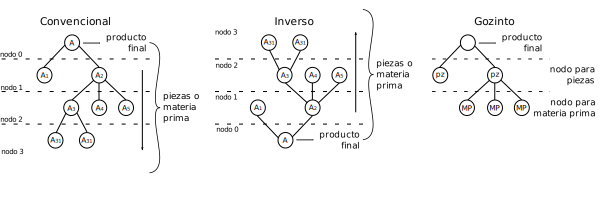
\includegraphics[scale=0.20]{Manufactura Integrada por Computadora Figuras/Figura04 Estructura del Producto.png}
        \caption{Estructura del producto}
    \end{figure}
    
    \item Part Master Data: Una parte es un componente, ensamble, materia prima, producto terminado necesario para la fabricación. Por cada parte, un archivo que contenga los atributos:
    
    \begin{itemize}
        \item Identificadores:
            \begin{itemize}
                \item Número de parte.
                \item Código.
            \end{itemize}
        \item Nombre.
        \item Descripción. 
        \item Tipo:
            \begin{itemize}
                \item Producto terminado.
                \item Ensamble. 
                \item Materia prima.
            \end{itemize}
        \item Unidad de medida:
            \begin{itemize}
                \item Pieza. 
                \item Kilogramo.
                \item Litro.
                \item Bulto.
            \end{itemize}
        \item Tipo de producción:
            \begin{itemize}
                \item Interna.
                \item Externa.
            \end{itemize}
        \item Tiempo de remplazo: refaccionamientos, tiempo de vida de los componentes.
        \item Fecha ultima de modificación.
        \item Fecha desde que es valido.
        \item Fecha de vigencia.
        \item Fecha de creación. 
        \item Persona encargada \( \to \) HRM
    \end{itemize}
\end{enumerate}

\subsection{Lista de materiales: BOM}

Representa la estructura del producto con la información esencial, se presenta en una tabla. Se debe identificar s las partes son continuas (ml, gr, kg) o discreta (pieza, pizca). 
Variante del producto: Productos finales con algunas modificaciones al modelo básico. 

\begin{table}[h]
    \centering
    \begin{tabular}{|c|c|c|c|c|c|c|c|}
        \hline
        código & variante & nivel & Part ID & nombre & descripción & unidad & cantidad \\
        \hline
         & & & & & & & \\
        \hline
    \end{tabular}
    \caption{Estructura BOM multinivel}
\end{table}

\subsection{Tipos de variante}
\begin{itemize}
    \item Estructura: Cambio significativo.
    \item Cantidad: Cuando se modifica la cantidad.
    \item Opcionales: Cuando se agregan partes al producto. 
    \item Internas: No tienen un cambio evidente en el producto, por ejemplo, cambio de proveedor. 
\end{itemize}

\subsection{Códigos de partes}
Se emplean para identificar las partes 
\begin{enumerate}
    \item Identificación: identifica un objeto.
    \item Clasificación: categoriza las partes:
        \begin{itemize}
            \item Compuesto: identifica y clasifica al mismo tiempo.
            \item Paralelo: identifica y clasifica, pero de forma separada.
        \end{itemize}
\end{enumerate}

\subsection{Plan maestro de producción}

La demanda de los productos finales se puede organizar un plan de ventas abstracto o por órdenes completas. 

Demanda: Cantidad y calidad de bienes y servicios que pueden ser adquiridos. Conjunto de consumidores. 

\begin{table}[h]
    \centering
    \begin{tabular}{|c|c|c|c|c|c|c}
        \hline
        periodo \( j \) & \( \cdots \) & 4 & 5 & 6 & 7 & \( \cdots \) \\
        \hline
        demanda \( m_{i} \) & \( \cdots \) & 100 & 50 & 20 & 200 & \( \cdots \) \\
        \hline
    \end{tabular}
    \caption{Demanda}
\end{table}

La demanda se puede estimar o aproximar. Depende si tienes ordenes concretas y un registro que permita la estimación. Una forma de estimarla es la siguiente:
\[
    V_{k} = V_{k-1} + \alpha (m_{k-1} - V_{k-1})
\]

Donde \( \alpha \) es el índice de la demanda \( 0 < \alpha < 1 \), \( m_{k} \) es la demanda actual y \( V_{k} \) es el valor pronostico. 

\subsection{Requerimientos para producción}
\begin{itemize}
    \item Requerimientos primarios: Se refiere a los productos terminados, es el punto inicial de la planeación de lo requerimientos.
    
    \item Requerimientos secundarios: Se refiere a productos intermedios, materia prima, consumibles. Es lo que se necesita para los requerimientos primarios. Se obtienen las cantidades requeridas según la demanda. 
\end{itemize}

\subsection{Determinar las condiciones de los proveedores o la manufactura}

\begin{itemize}
    \item Unidad: Como la usa la empresa.
    \item Restricción: Como nos venden los proveedores.
\end{itemize}

\begin{table}[h!]
    \centering
    \begin{tabular}{|c|c|c|c|}
        \hline
        parte & descripción & unidad & restricción \\
        \hline
         &  &  &  \\
    \end{tabular}
    \caption{Demanda}
\end{table}

\subsection{Inventarios: JIT}

\[
\begin{split}
    R & = \text{Reorder point} \\
    Z & = \text{Safety stock (inventario de seguridad)} \\
    Q & = Order quantity \\
    t_{w} & = Lead time (tiempo de entrega, para abastecer) \\
    t_{z} & = Safety time (tiempo de seguridad, aun se puede producir)
\end{split}
\]

\begin{figure}[h!]
    \centering
        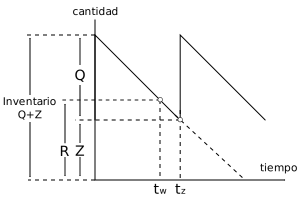
\includegraphics[scale=0.25]{Manufactura Integrada por Computadora Figuras/Figura05 Just in Time.png}
        \caption{JIT}
\end{figure}

\subsection{Diagrama de ensamble: Assembly chart}

Representa las operaciones de transformación y ensamble de las partes para conformar un producto. 
\begin{itemize}
    \item F: Fabricación
    \item E: Ensamble
    \item A: Adquisición
    \item P: Procurement
    \item RW: Raw Material
    \item F: Fabrication
    \item A: Assembly
\end{itemize}

\begin{figure}[h!]
    \centering
        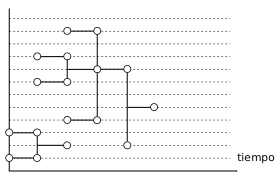
\includegraphics[scale=0.25]{Manufactura Integrada por Computadora Figuras/Figura06 Diagrama de Ensamble.png}
        \caption{Diagrama de ensamble}
\end{figure}

\subsection{MRP}
\begin{figure}[h!]
    \centering
        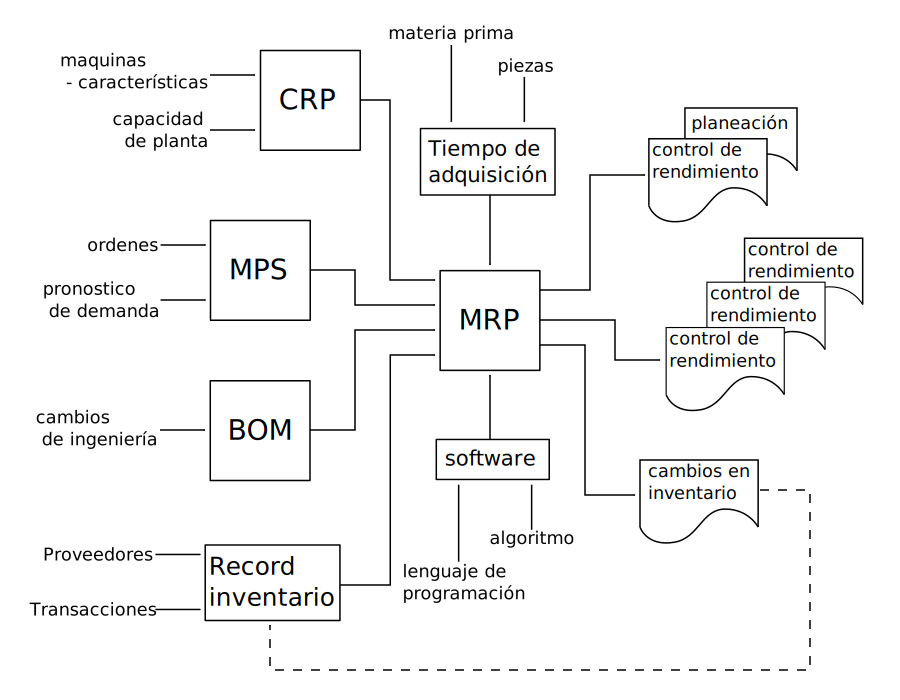
\includegraphics[scale=0.15]{Manufactura Integrada por Computadora Figuras/Figura07 MRP.png}
        \caption{MRP}
\end{figure}